\section{Our Method}
\label{sec:method}

The workflow of our method is illustrated in Figure~\ref{fig:pipeline}.  
From the fusion simulations, we first precondition the data with the robust principal component analysis (RPCA)~\cite{CandesLMW11}, and then use the topology analyses to extract blobs as connected components of critical points (local minima/maxima).  The blobs are further tracked over different timesteps.  The dynamics of the blobs, such as birth/death/merge/split events are further visualized for fusion scientists to analyze the data.  


% We first load the output scalar electrostatic potential field from ADIOS I/O, 

\begin{figure}
  \centering
  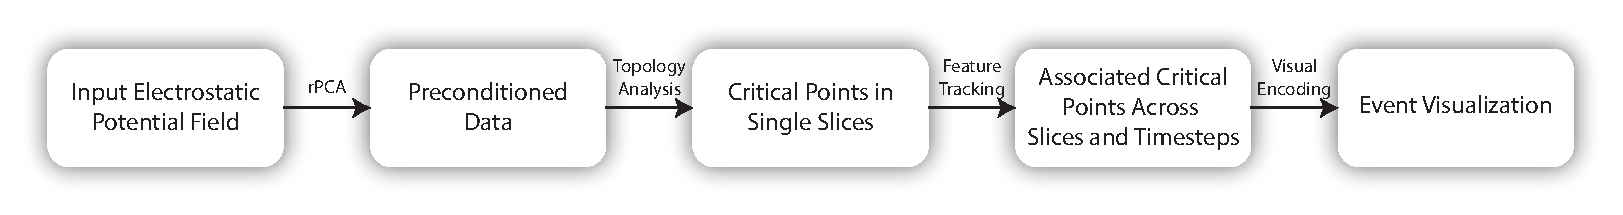
\includegraphics[width=\linewidth]{Figs/pipeline}
  \caption{The pipeline of our method.}
  \label{fig:pipeline}
\end{figure}


\subsection{Data preconditioning}

We use the RPCA to precondition the time series data, in order to distinguish the moving and stationary patterns as ``foregrounds'' and ``backgrounds.''  Formally, the input data matrix $M$ can be decomposed as 

\begin{equation}
M = L_0 + S_0, 
\end{equation}

\noindent where $L_0$ has low rank and $S_0$ is a sparse perturbation matrix.  RPCA has been used to identify activities in video surveillance data, so that $L_0$ and $S_0$ correspond to the stationary background and moving features, respectively.  By preconditioning the input time series, we can detect the moving features for further blob tracking.  We are working with George Ostrouchov and Jong Choi from ORNL to generalize this technique to precondition the triangular mesh data.  


\subsection{Blob extraction}

%\begin{figure}[!h]
%  \centering
%  \includegraphics[width=\linewidth]{Figs/blobs}
%  \caption{(a) Blob tracking over slices and time; (b) critical point tracking based on the combinatorial feature flow fields (image courtesy Reininghaus et al.~\cite{ReininghausKWH12})}
%  \label{fig:blob}
%\end{figure}

\begin{figure}
  \centering
  \includegraphics[width=\linewidth]{Figs/simplification2D}
  \caption{Topology simplification of a 2D slice with three different persistence thresholds: (a) and (d) 0, (b) and (e) 20, (c) and (f) 40.  The simplified scalar field are visualized in (a), (b), and (c), and the corresponding segmentation results are shown in (d), (e), and (f).}
  \label{fig:simplification2D}
\end{figure}


In this study, blobs are defined as topological segmentations of Reeb graphs.  Based on the concepts reviewed in Section~\ref{sec:topology}, in order to extract comprehensive topological information, we need Reeb graphs instead of contour trees, because the torus-shaped 3D domain is non-simply connected.  However, in our current prototype implementation, we are still using contour trees for proof of concept.  We will replace contour trees with Reeb graphs in the next milestones of this project.  Unless otherwise noted, the following discussions are based on contour trees instead of Reeb graphs.  

The contour tree construction is a multistage process~\cite{CarrSA00}.  First, we sort all vertices in an array based on the scalar values monotonously from the global minimum to the global maximum.  Second, we sweep the array downwards and upwards to construct the \emph{join tree} and the \emph{split tree}, respectively.  Details of the join/split constructions are documented in~\cite{CarrSA00}.  Third, we merge the join tree and split tree to form the contour tree.  The topological segmentation is then achieved by associating the vertices to the arcs of the contour tree.  

The contour tree must be simplified to identify meaningful blobs in practice, because the fluctuation of the turbulence will generate many meaningless local maxima/minima, as shown in Figure~\ref{fig:simplification2D}.  We currently use persistence~\cite{EdelsbrunnerLZ02} as the criteria to merge arcs and thus to simplify contour tree.  As reviewed in Section~\ref{sec:topology}, persistence is defined as the difference between saddle and min/max values of an arc.  By pruning arcs with least persistence values, we can obtain a smaller set of blobs for further exploration.  

In our current implementation, we follow Pascucci et al.~\cite{Pascucci2004} to use branch decomposition---an alternative representation of contour trees---to simplify contour trees.  First, we transform the input contour tree to a branch decomposition tree.  Second, we prune branches in the branch decomposition tree by a given persistence threshold.  Third, we transform the pruned branch decomposition tree back to the simplified contour tree.  

Figure~\ref{fig:simplification2D} visualizes topological segmentation results of a single slice dataset with different persistence thresholds.  The results without simplifications (threshold equals to zero) are shown in the first column; all local minima/maxima are kept.  The second and third column are the results with the persistence threshold 20 and 40, respectively.  We can see that the simplification keeps most salient blob features in the data.  


% As illustrated in Figure~\ref{fig:blob}(a), in our study, blob detection is defined as the extraction of critical points (local minima and maxima) in 2D slices; blob tracking is defined as associating blobs across different planes and different timesteps.  The critical point tracking is based on the combinatorial feature flow fields method~\cite{ReininghausKWH12}, which is a generalization of a feature flow field~\cite{TheiselS03} in the combinatorial sense.  We are also going to use merge tree theories to simplify the blob detection and tracking results~\cite{OesterlingHWMS17}.  3D visualizations will be provided to explore the spatiotemporal distributions of the tracked blobs.  


\subsection{Blob tracking}

We are going to explore two distinct approaches to track the evolution of blobs over time, including region overlap and time-varying topologies.  The output of either approach is a \emph{tracking graph}.  The nodes in the tracking graph are individual blobs in all timesteps.  Two nodes in the adjacent timesteps are linked, if they are associated temporally.  

In the region overlap approach~\cite{SilverW98}, two blobs in the adjacent timesteps are associated if they have significant spatial overlaps.  The saliency can be defined by the percentage of overlaps or other geometric measurements.  

In the time-varying topology approach~\cite{SohnB06}, we will need to extract Reeb graphs or contour trees in both space and time.  In this case, each blob will be a spatiotemporal object and thus blob tracking is automatically achieved.  

In both cases, the tracking graph will be obtained and then we can further define events for analysis and visual exploration.  The event visualization is discussed in the following section.  


\subsection{Event visualization}

\begin{figure}
  \centering
  \includegraphics[width=\linewidth]{Figs/events}
  \caption{Proposed event visualization of blobs (image courtesy Scott Klasky, ORNL)}
  \label{fig:events}
\end{figure}

We are going to develop new visualizations for fusion scientists to understand the dynamics of the blobs.  We will define several different types of events, including birth, death, merge, and split to characterize the behaviors of blobs.  In our previous study of magnetic flux vortex tracking~\cite{GuoPPKG16, GuoPG17, PhillipsGPKG16, PhillipsPKG15}, we have already developed a graph-based representation of such events.  We are going to further generalize the previous methods to visualize the events in the XGC data.  

\begin{figure}
  \centering
  
\includegraphics[width=\linewidth]{Figs/storyline}
  \caption{Proposed storyline visualization of blob merge/split events (image courtesy Guo et al.~\cite{GuoPPKG16})}
  \label{fig:storyline}
\end{figure}

The design of the event visualization, which is inspired by storyline visualization~\cite{TanahashiM12} is illustrated in Figure~\ref{fig:storyline}.  The event visualization gives an overview of blob dynamics over time.  In this view, each colored ribbon represents one blob.  The duration of the blob is encoded by the length of the ribbon.  Blobs are connected to each other with short gray lines if the blobs are involved in an merge/split event.  User interactions including zooming and panning are provided for users to dig into details in the long time sequence.  

In the existing design, the graph layout implementation is based on the \texttt{dot} algorithm provided by the Graphviz package~\cite{GansnerN00}.  We minimize the number of crossings in the graph layout in order to reduce visual clutters and to increase the readability.  An automatic color scheme is also generated to avoid visual ambiguities based the two constrains: (1) blobs that appear in the same time spans must have different colors; (2) blobs involved in the same merge/split event must have different colors.  The generated graph layout will be visualized in a web-based user interface for interactive exploration. 


% 

% Critical point tracking~\cite{ReininghausKWH12}.

% 

% Feature flow fields~\cite{TheiselS03}. 
